\documentclass{standalone}
\usepackage{tikz}
\usetikzlibrary{positioning}
\begin{document}
	
	
	
	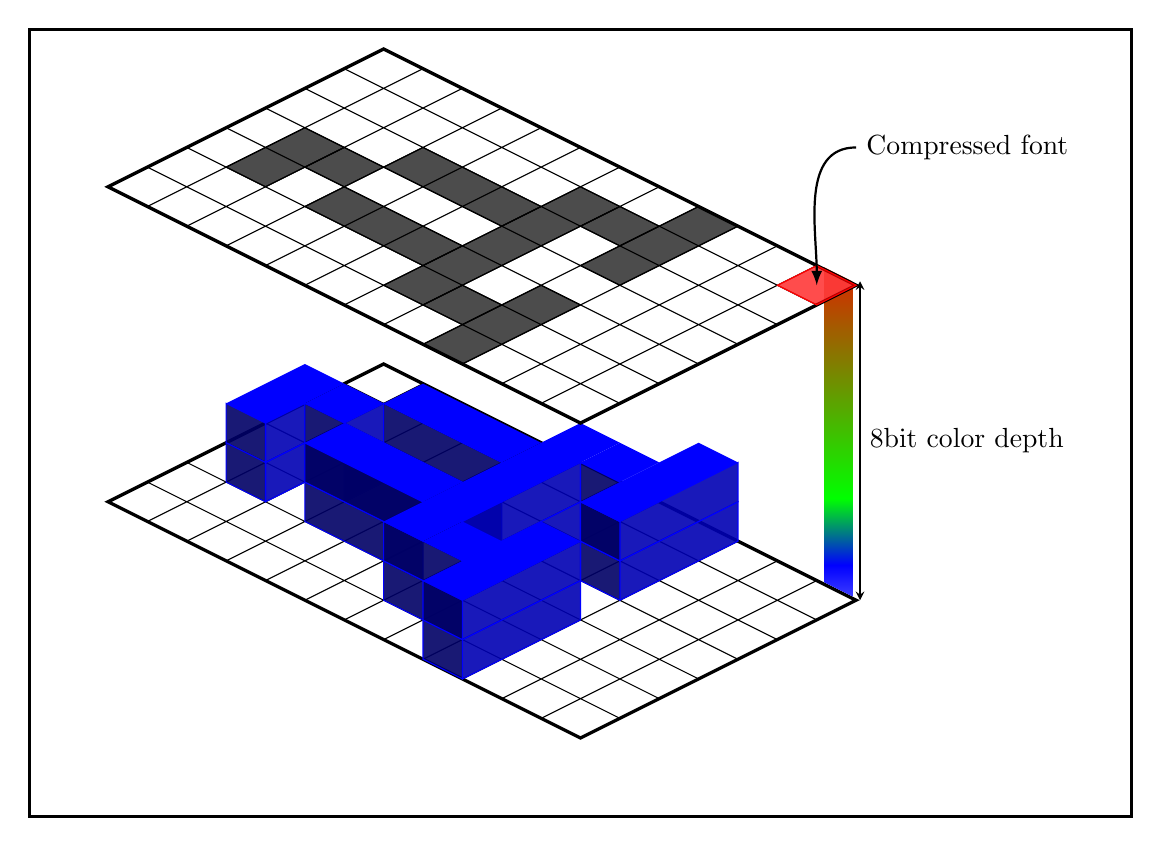
\begin{tikzpicture}[scale=.5,every node/.style={minimum size=1cm},on grid]
	\begin{scope}%
	\draw[very thick] (-14,-10) rectangle (14,10);
	
	%slanting: production of a set of n 'laminae' to be piled up. N=number of grids.
	\begin{scope}[
	yshift=-80mm,every node/.append style={
		yslant=0.5,xslant=-1},yslant=0.5,xslant=-1
	]
	% opacity to prevent graphical interference
	\fill[white,fill opacity=0.9] (0,0) rectangle (7,12);
	\draw[step=10mm, black] (0,0) grid (7,12); %defining grids
	%\draw[step=1mm, red!50,thin] (3,1) grid (4,2);  %Nested Grid
	\draw[black,very thick] (0,0) rectangle (7,12);%marking borders
	%\fill[red] (0.05,0.05) rectangle (0.35,0.35);
	%Idem as above, for the n-th grid:
	\end{scope}
	
		\definecolor{C0}{RGB}{255,255,255}
	\definecolor{C1}{RGB}{0,0,255}
	\definecolor{C2}{RGB}{0,255,0}
	\definecolor{C3}{RGB}{255,0,0}
	\pgfdeclareverticalshading{someShading}{40bp}{
		color(-10bp)=(C0);
		color(10bp)=(C1);
		color(20bp)=(C2);
		color(60bp)=(C3)
	} 
	\shade [shading=someShading](7,3.55)--(7,-4.45) -- (6.1,-4)--(6.1,4)--(7,3.55);
	

	
	\foreach \r in {-80,-70}{
	\begin{scope}[
	yshift=\r mm,yslant=0.5,xslant=0
	]
	\draw[blue,fill opacity=.9,fill=black!30!blue] (0,3) rectangle (-3,4);
	\draw[blue,fill opacity=.9,fill=black!30!blue] (1,3) rectangle (4,4);
	\draw[blue,fill opacity=.9,fill=black!30!blue] (-3,5) rectangle (0,6);
	\draw[blue,fill opacity=.9,fill=black!30!blue] (-6,9) rectangle (-5,10);
	\draw[blue,fill opacity=.9,fill=black!30!blue] (-8,10) rectangle (-7,11);
	\end{scope}
	

	\begin{scope}[
	yshift=\r mm,yslant=-0.5,xslant=0
	]
	\draw[blue,fill opacity=.9,fill=black!60!blue] (-3,1) rectangle (-4,0);
	\draw[blue,fill opacity=.9,fill=black!60!blue] (-3,2) rectangle (-5,1);
	\draw[blue,fill opacity=.9,fill=black!60!blue] (-4,3) rectangle (-7,2);
	\draw[blue,fill opacity=.9,fill=black!60!blue] (-4,4) rectangle (-7,3);
	\draw[blue,fill opacity=.9,fill=black!60!blue] (-8,3) rectangle (-9,2);
	\draw[blue,fill opacity=.9,fill=black!60!blue] (1,4) rectangle (-0,5);
	\draw[blue,fill opacity=.9,fill=black!60!blue] (1,5) rectangle (-0,6);
	\draw[blue,fill opacity=.9,fill=black!60!blue] (-5,4) rectangle (-2,5);
	\end{scope}	
	
}
	\begin{scope}[
	yshift=-60mm,yslant=0.5,xslant=-1
	]
	%\draw[red,fill opacity=.8,fill=black] (1,1) rectangle (0,0);
	\fill [blue] (0, 3) rectangle (3, 4);
	\fill [blue] (4, 3) rectangle (7, 4);
	\fill [blue] (1, 4) rectangle (2, 5);
	\fill [blue] (5, 4) rectangle (6, 5);
	\fill [blue] (1, 5) rectangle (6, 6);
	\fill [blue] (2, 6) rectangle (3, 9);
	\fill [blue] (4, 6) rectangle (5, 9);
	\fill [blue] (3, 9) rectangle (4, 10);
	\fill [blue] (2, 10) rectangle (4, 11);
	\end{scope}	
	
	
	
	\begin{scope}[
	yshift=0mm,every node/.append style={
		yslant=0.5,xslant=-1},yslant=0.5,xslant=-1
	]
	\fill[white,fill opacity=.7] (0,0) rectangle (7,12);
	\draw[black,very thick] (0,0) rectangle (7,12);
	\draw[step=10mm, black] (0,0) grid (7,12);
	
	\draw[red,fill opacity=.7,fill=red] (6, 0) rectangle (7, 1);
	
	\draw[black,fill opacity=.7,fill=black] (0, 3) rectangle (3, 4);
	\draw[black,fill opacity=.7,fill=black] (4, 3) rectangle (7, 4);
	\draw[black,fill opacity=.7,fill=black] (1, 4) rectangle (2, 5);
	\draw[black,fill opacity=.7,fill=black] (5, 4) rectangle (6, 5);
	\draw[black,fill opacity=.7,fill=black] (1, 5) rectangle (6, 6);
	\draw[black,fill opacity=.7,fill=black] (2, 6) rectangle (3, 9);
	\draw[black,fill opacity=.7,fill=black] (4, 6) rectangle (5, 9);
	\draw[black,fill opacity=.7,fill=black] (3, 9) rectangle (4, 10);
	\draw[black,fill opacity=.7,fill=black] (2, 10) rectangle (4, 11);
	
	\end{scope}
	
	%putting arrows and labels:
	\draw[-latex,thick] (7,7) node[right]{Compressed font}
	to[out=180,in=90] (6,3.5);
	
	\draw[<->,>=stealth](7.1,3.6)--(7.1,-4.5) node[midway,right] {8bit color depth};
	
	%\draw[-latex-,thick] (-3+14,2.5-9)to(-1.2+14,1-9);
	
	%drawing points on grid's conrners.
	\end{scope}
	\end{tikzpicture}
	
\end{document} 